\subsection{Growing the box by adding a new partition}
\label{sec:sdm_grow}	
	
In this SDM, we shall specify how our learning box is built up and how the
contained partitions are connected.  This controls how cards move back and
forward in the box.  Although very different behaviour can be implemented, we
shall implement the classical rules as depicted in
Fig.~\ref{fig:membox_illustration}.

Start off by creating the simple control flow and story pattern depicted in
Fig.~\ref{fig:sdm_grow_1}.  This matches the box itself (\texttt{this}), and
\emph{any} two partitions in the box.
	
\begin{figure}[htp]
\begin{center}
  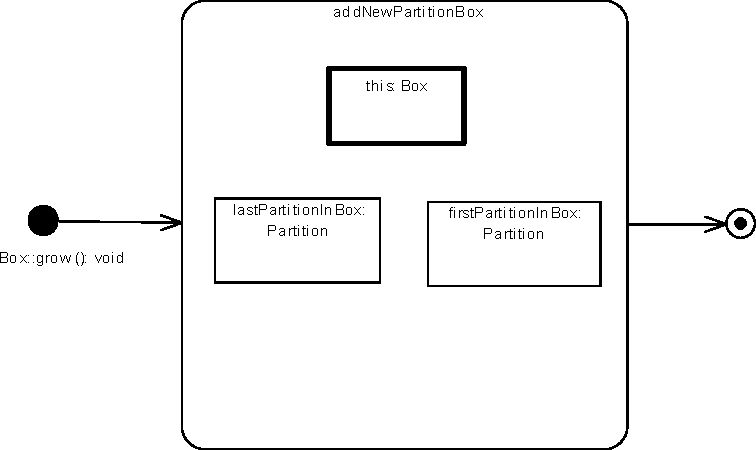
\includegraphics[width=0.7\textwidth]{pics/sdmBilder/grow/sdm57.pdf}
  \caption{Context elements for SDM.}  
  \label{fig:sdm_grow_1}
\end{center}
\end{figure}

As already indicated by the chosen names of the object variables
\texttt{first\-Partition} and \texttt{last\-Partition\-In\-Box}, we actually
want the pattern matcher to determine the first and the last partition in the box.
But how do we specify this?  As explained in section \ref{sec:empty}, the
current story pattern will simply determine two partitions
non-deterministically.  

SDMs provide a declarative means of identifying the first and last
partition via \emph{Negative Application Conditions}, also simply
referred to as \mbox{NACs}\footnote{Pronounced $\backslash 'nak \backslash$}.
A \mbox{NAC} is a negative element that should \emph{not} be present in a valid
\note{\mbox{NACs}}
match.  In the theory of algebraic graph transformations \cite{EEPT06},
\mbox{NACs} can be complex graphs that are much more general and powerful.  In
our implementation\footnote{To be more precise CodeGen2 from Fujaba.}, however,
we only support single negative elements (object or link variables).

To create an appropriate \mbox{NAC} that constrains the possible matches for
\texttt{lastPartitionInBox} to exactly the last partition in the box, create a
new object variable \texttt{nextPartition} of type \texttt{Partition} and set
\note{Binding Semantics}
its \emph{Binding Semantics} to \texttt{negative} (Fig.~\ref{fig:sdm_grow_2}).  
The object variable should be visualised as being cancelled or struck out.
 
\begin{figure}[htbp]
\begin{center}
  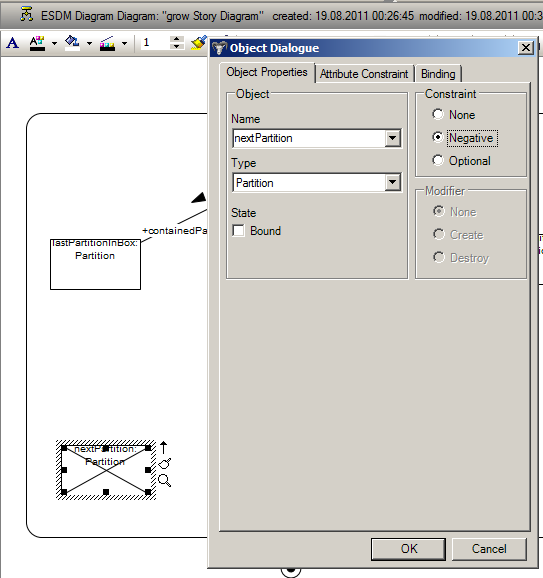
\includegraphics[width=0.7\textwidth]{pics/sdmBilder/grow/sdm58RAW}
  \caption{Adding a negative element.}  
  \label{fig:sdm_grow_2}
\end{center}
\end{figure}
 
Now quick link \texttt{nextPartition} to \texttt{lastPartitionInBox} and choose
the link type carefully, so that \texttt{nextPartition} plays the role of
\texttt{next} with respect to \texttt{lastPartitionInBox}.  Now complete the
story pattern so that it closely resembles Fig.~\ref{fig:sdm_grow_3}.  The
\mbox{NACs} can be interpreted as follows:  The first/last partition in the box
is \emph{a} partition in the box that has no previous/next partition.  The
valid matches are made unique and thus deterministic by construction, i.e., if
you \emph{grow} the box via this method, there will always be exactly one first
and one last partition.  

\begin{figure}[htbp]
\begin{center}
  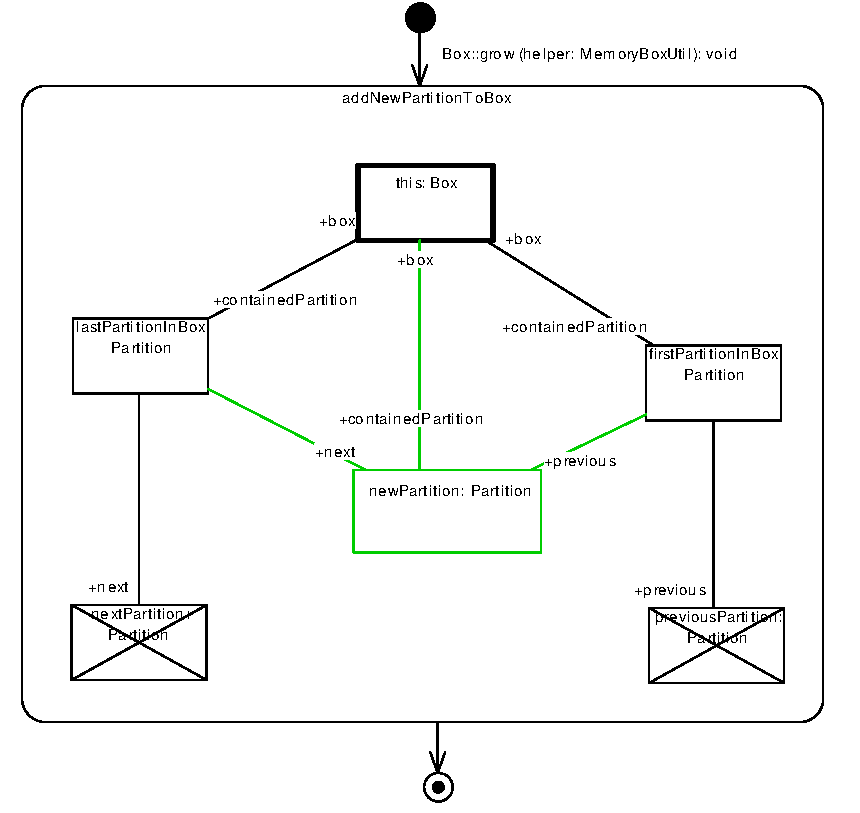
\includegraphics[width=0.7\textwidth]{pics/sdmBilder/grow/sdm65}
  \caption{Determining the first and last partition with NACs.}  
  \label{fig:sdm_grow_3}
\end{center}
\end{figure}
 
Note how the newly created partition
\texttt{newPartition} is hung into the box (it becomes the next partition of the
current last partition and has as its previous partition the first partition
in the box) according to the arrows in Fig.~\ref{fig:membox_illustration}.
  
All that is missing to complete our SDM is an assignment to set the size of the
new partition.  We already know that an assignment is an attribute
constraint with \texttt{:=} as operator so go ahead and invoke the corresponding
dialogue.  As the new size must be calculated depending on the rest of the
partitions in the box (partitions usually get bigger) we call a helper function
\note{MethodCallExpression}
via a \emph{MethodCallExpression}.  A MethodCallExpression is used to invoke a
method that is defined in a class in the current EA project.  Enter the values
in Fig.~\ref{fig:sdm_grow_4} choosing the argument \texttt{helper} as target and
\texttt{determineNextSize} as the method to be invoked.  Parameters can be
specified by just choosing the appropriate parameter declaration between
guillemets (e.g. \texttt{<Box box>}) via the drop-down menu and typing in the
value (this is basically a literal expression). So, be sure that \texttt{<Box box>} is selected
from the drop down menu and replace its text with \texttt{this}. Don't forget to
press the \texttt{Save} button for every parameter and \texttt{Add} 
+ \texttt{OK} to confirm and close the dialogue.
 
\begin{figure}[htbp]
\begin{center}
  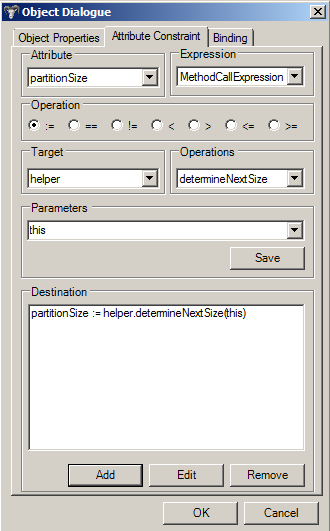
\includegraphics[width=0.25\textwidth]{pics/sdmBilder/grow/sdm66}
  \caption{Invoking a method via a \texttt{MethodCallExpression}.}  
  \label{fig:sdm_grow_4}
\end{center}
\end{figure}

If you've done everything right, your SDM should now closely resemble
Fig.~\ref{fig:sdm_grow_5}.  As usual, try to export, generate code, inspect the
method implementation and write a JUnit test.  This time around you also have to
implement the helper method \texttt{determineNextSize} directly in the
generated code
(\texttt{gen/\-LearningBoxLanguage/\-facade/\-impl/\-LearningBoxUtilImpl}).
Don't forget to add \texttt{@generated NOT} to the Java doc comment of the
method so the code generator preserves your code in future runs.
When testing (which you will \emph{of course} do right?), note that you can only grow a ``minimal'' box that has at least a first and last partition, i.e., a box with no partitions at all cannot be grown using our specified SDM. 

\begin{figure}[htbp]
\begin{center}
  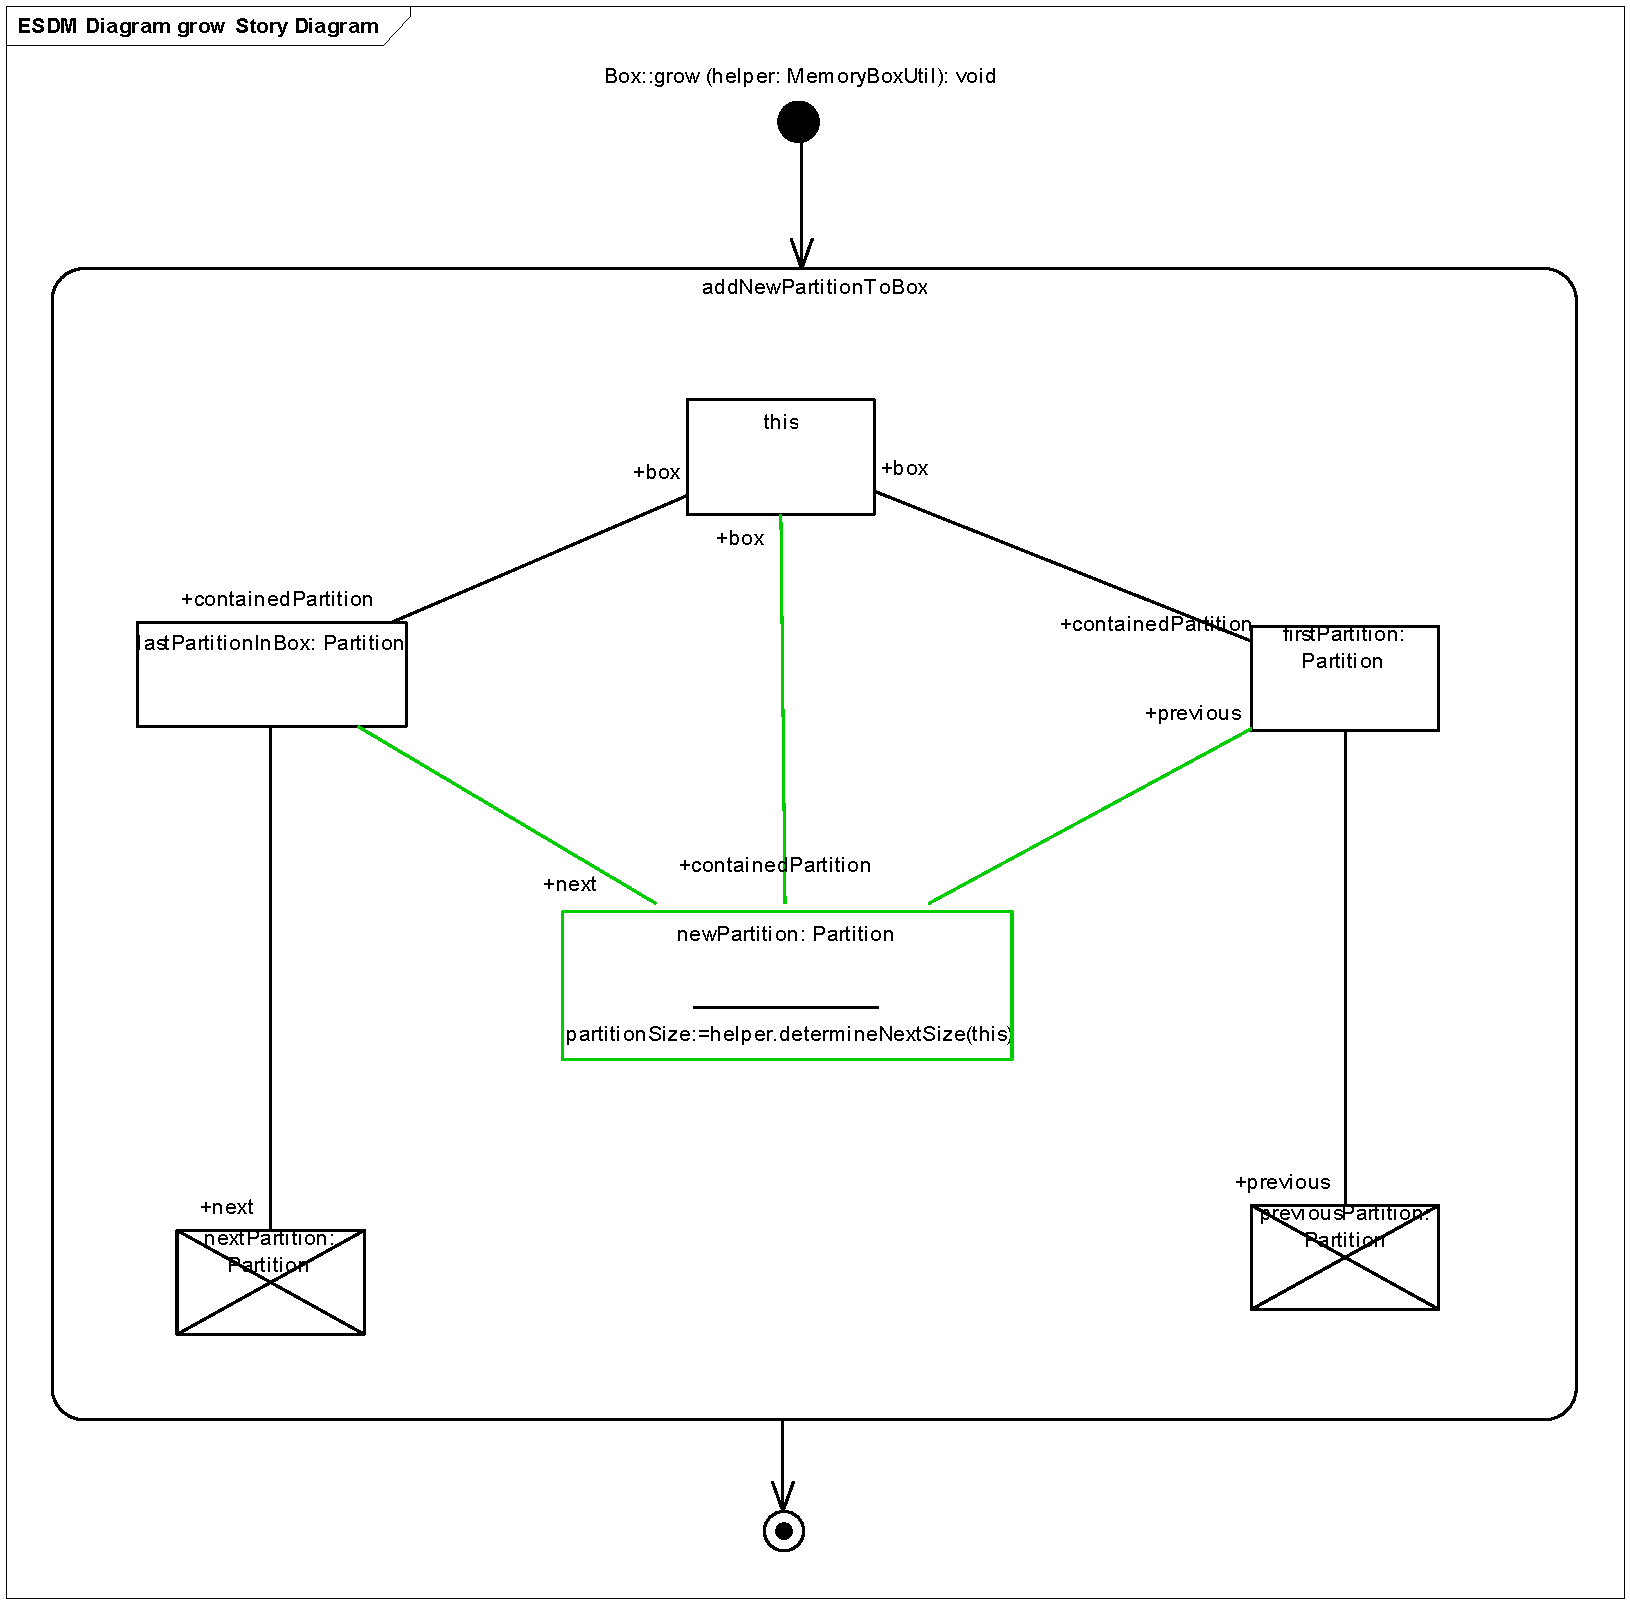
\includegraphics[width=0.75\textwidth]{pics/sdmBilder/grow/sdm67}
  \caption{Complete SDM for \texttt{Box::grow}.}  
  \label{fig:sdm_grow_5}
\end{center}
\end{figure}
